\chapter{Materials and Methods}

\section{Patients characterization}

This study is part of the research project entitled "Clinical utility of liquid biopsy in non-small cell lung cancer patients with EML4-ALK translocation". Its objective is to determine the best strategy for the identification of EML4-ALK translocations and to assess the clinical utility of periodic tumor monitoring in ALK-positive NSCLC patients from liquid biopsies. In this context, between June 2015 and July 2019, several ALK-positive NSCLC advanced subjects were recruited from 6 hospitals across Spain, including the Hospital Universitario Puerta de Hierro, the Complejo Hospitalario Universitario A Coruña, the Hospital Universitario Fundación Jiménez Díaz, the Hospital Clínic Barcelona, the Hospital General Universitario de Alicante, and the Hospital General Universitario de Valencia.

The primary study was conducted under the precepts of the Helsinki Declaration and was approved by the Hospital Puerta de Hierro Ethics Committee (internal code 79-18). Patients were eligible if they consented to allow their clinical information to be used in the previously mentioned research project. Their clinical history was queried for information on the age of diagnosis, sex, smoking status, histology, Eastern Cooperative Oncology Group (ECOG) status at the start of the study, stage, previous therapies, and date of death.

Eligible patients had histologically confirmed diagnosis of stage III–IV NSCLC that was ALK-positive, a measurable disease according to the response evaluation criteria in solid tumors (RECIST, version 1.1), were candidates to be treated with an ALK inhibitor, and were 18 years old or older. Exclusion criteria included the impossibility of frequent venipuncture or evidence of any other major clinical disorder or finding that would have made it undesirable for the patient to participate in the study.

\section{Laboratory Procedures}

To obtain the necessary data to develop the automatic algorithm for filtering genetic variants, a series of clinical procedures have been carried out, including the preparation and conditioning of the samples, their sequencing and analysis, and the subsequent confirmation of the ALK-positive samples.

\subsection{Sample Collection and Conditioning}

Once the EML4-ALK translocation has been diagnosed in a patient with NSCLC according to an anatomic pathology report (FISH and\slash or IHC), peripheral blood is extracted in a 9 $mL$ Streck Cell-Free DNA BCT\textsuperscript\textregistered{} (Streck, USA) tube and transported to the Liquid Biopsy Laboratory, where it is preserved until its conditioning.

In this study, isolation of cfDNA and exosomes from the cellular fraction was achieved by two consecutive centrifugation processes at room temperature, the first at 1500 $g$ for 10 $min$ and the second at 5000 $g$ for 20 $min$. After discarding the supernatant containing the clean plasma, cfDNA and exosome RNA isolation was performed using the QIAamp\textsuperscript\textregistered{} Circulating Nucleic Acid Kit (QIAgen, Valencia, CA, USA) and the exoRNeasy\textsuperscript\textregistered{} Serum/Plasma Maxi Kit (QIAgen, Valencia, CA, USA) respectively, following the manufacturer's instructions. Until library preparation for sequencing, conditioned samples were stored at $-80$ \textdegree{C}.

Within the context of the project in which this thesis is included, blood samples have been extracted from patients in the pre-treatment stage, at months 2, 4, 6, 8, 12, 15 and 18, and at progression.

\subsection{Library Preparation}

Libraries were prepared from 10.4 $\mu L$ of cfDNA or exosome RNA using the Oncomine\texttrademark{} Pan-Cancer Cell-Free Assay (Thermo Fisher, Palo Alto, CA, USA) according to the manufacturer's instructions. This multi-biomarker amplicon-based assay is optimized to detect more than 900 hotspots in 52 key genes from liquid biopsy samples containing tumor-derived DNA and RNA. It enables a limit of detection (LOD) down to 0.1\%, allowing the study of single nucleotide variants (SNVs), short insertions or deletions (indels), copy number variations (CNVs), and fusions. Specifically, the subsequent steps have been followed to prepare the NGS libraries (\autoref{fig:library}):

\begin{figure}[ht]
    \centering
    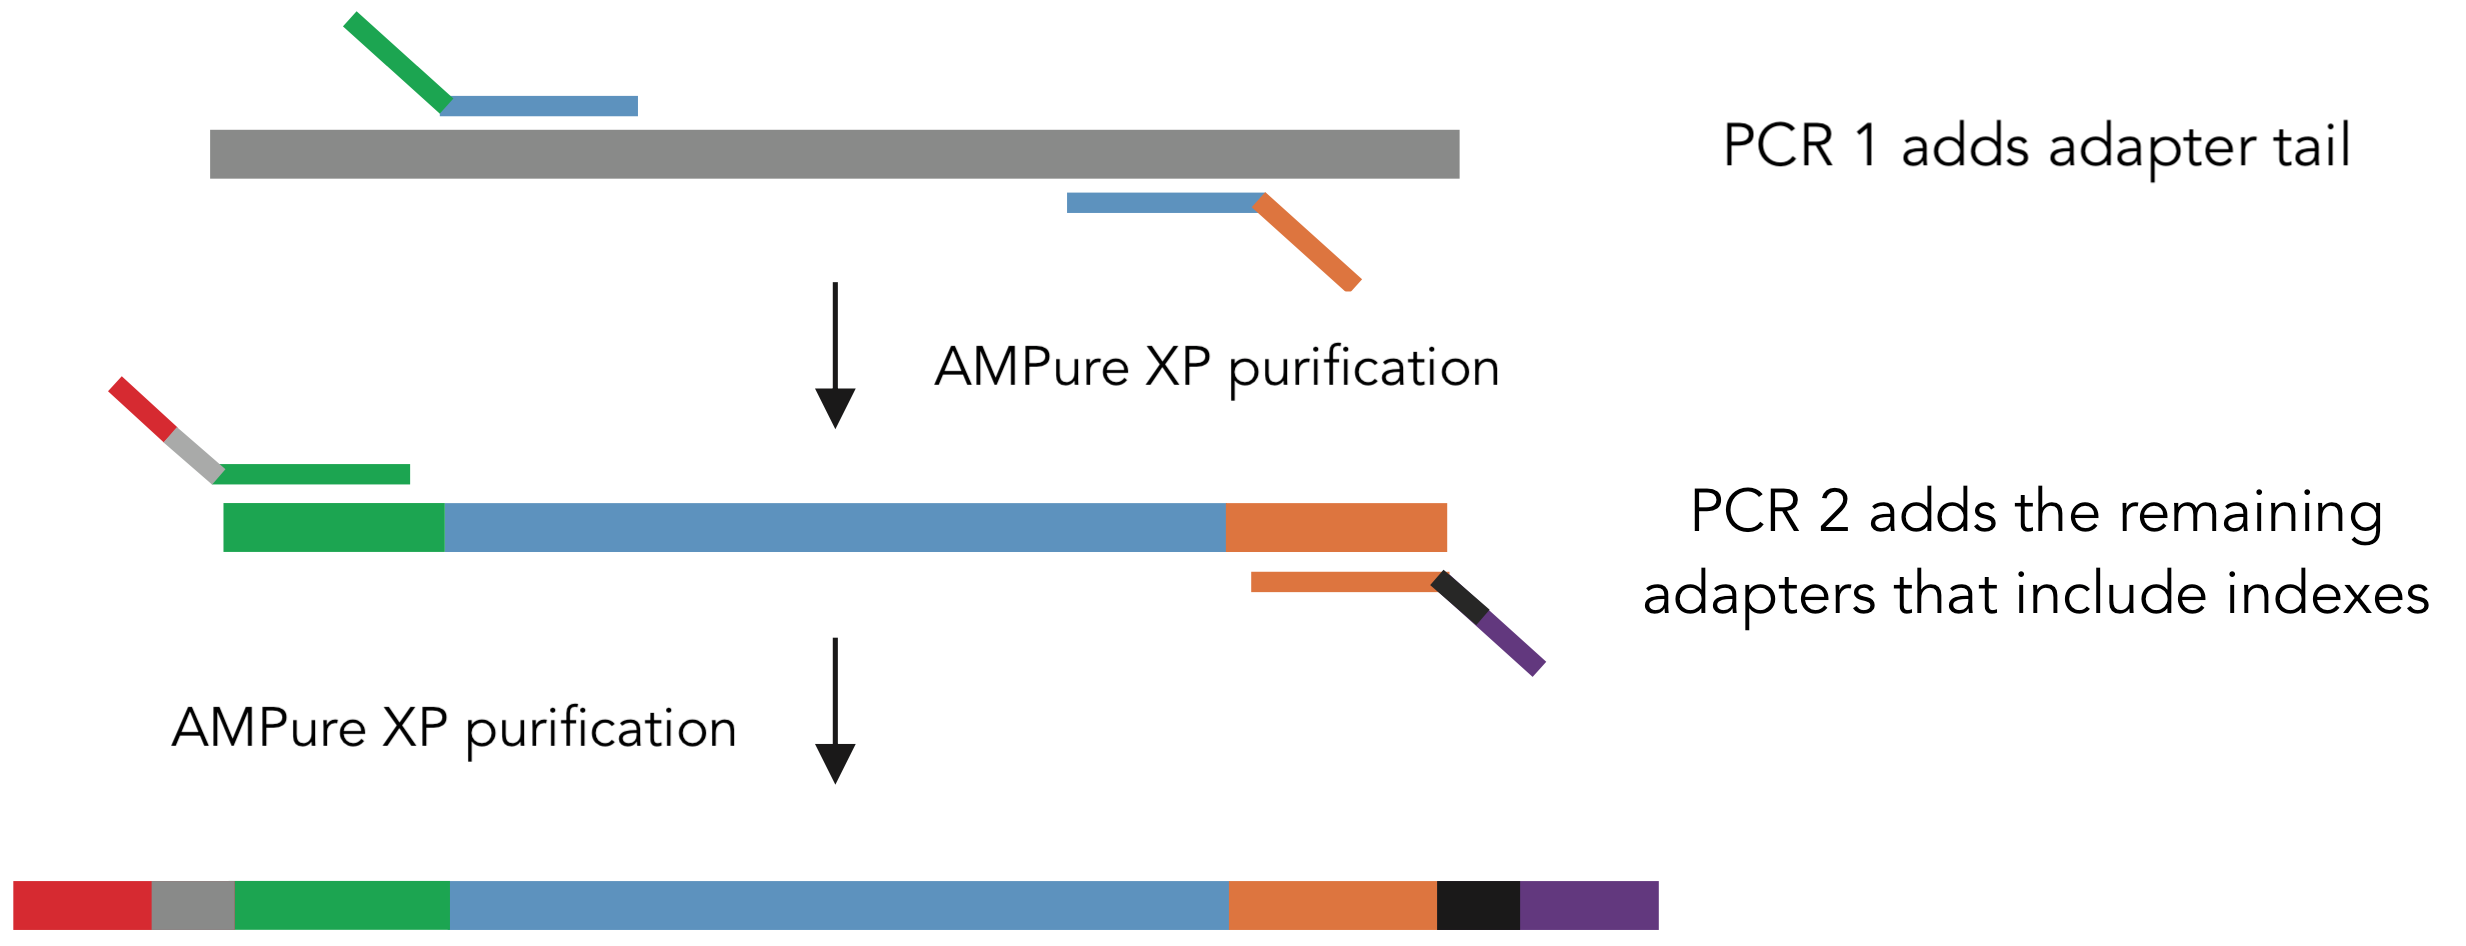
\includegraphics[width=0.85\textwidth]{Images/chapter_3/NGS_library.png}
    \caption{Amplicon-based library preparation.}
    \label{fig:library}
\end{figure}

\begin{enumerate}[font=\bfseries]
    \item \textbf{Reverse transcription of cell-free nucleic acids}. This step was only performed with exosome RNA samples, from which cDNA used for the following steps was synthesized.
    \item \textbf{Target amplification}. After the fragmentation of the isolated DNA using enzymatic methods, PCR amplification of these targets was used to produce labeled DNA amplicons within the desired size range.
    \item \textbf{Target amplicons purification}. Sample purification is a critical step for obtaining accurate NGS data. Therefore, in this study, a specific reagent with magnetic beads was used to remove short primers, unincorporated deoxyribonucleotide triphosphates (dNTPs), enzymes, short-failed PCR products, and salts from PCR fragments.
    \item \textbf{Amplification of the target amplicons with barcode adapted primers}. In this step, specific DNA adapter sequences were annealed to the 5' and 3' ends of the amplicon DNA. These adapters, among other functions, allow each sample to be marked with a specific nucleotide code, enabling the sequencer to analyze multiple patient samples simultaneously.
    \item \textbf{Barcoded library purification}. To guarantee reliable sequencing results, and in a process similar to the previous one, a purification of the labeled amplicons was carried out.
    \item \textbf{Size selection}. To isolate the DNA fragment sizes of interest for efficient and high-quality DNA sequencing, magnetic beads with varying concentrations of buffers were used in this step.
    \item \textbf{Library quantification}. To estimate the DNA concentration and to ensure equal representation of the indexed libraries, each of the samples was quantified with a qPCR and compared to the standard curve. Finally, the definitive barcoded libraries were pooled and adjusted to a final concentration of 50 $pM$.
\end{enumerate}

AMPure XP\textsuperscript\textregistered{} magnetic beads (Beckman Coulter, Inc., Brea, CA, USA) were used to carry out the purification and size selection steps, while the Ion Library TaqMan\texttrademark{} Quantitation Kit (Thermo Fisher, Palo Alto, CA, USA) and the StepOnePlus\texttrademark{} Real-Time PCR System (Thermo Fisher, Palo Alto, CA, USA) were used for the quantification.

\subsection{Template Preparation and Chip Loading}

Template preparation is based on an emulsion PCR (ePCR) method (\autoref{fig:ePCR}). It starts with the denaturation of the fragmented and ligated DNA, which is then mixed with beads. Each bead has thousands of copies of an oligonucleotide, which is complementary to one of the adapters and to which the corresponding DNA fragments are attached by clonal amplification. Empty beads are discarded and the rest are deposited into wells of a chip (one bead per well).

\begin{figure}[ht]
    \centering
    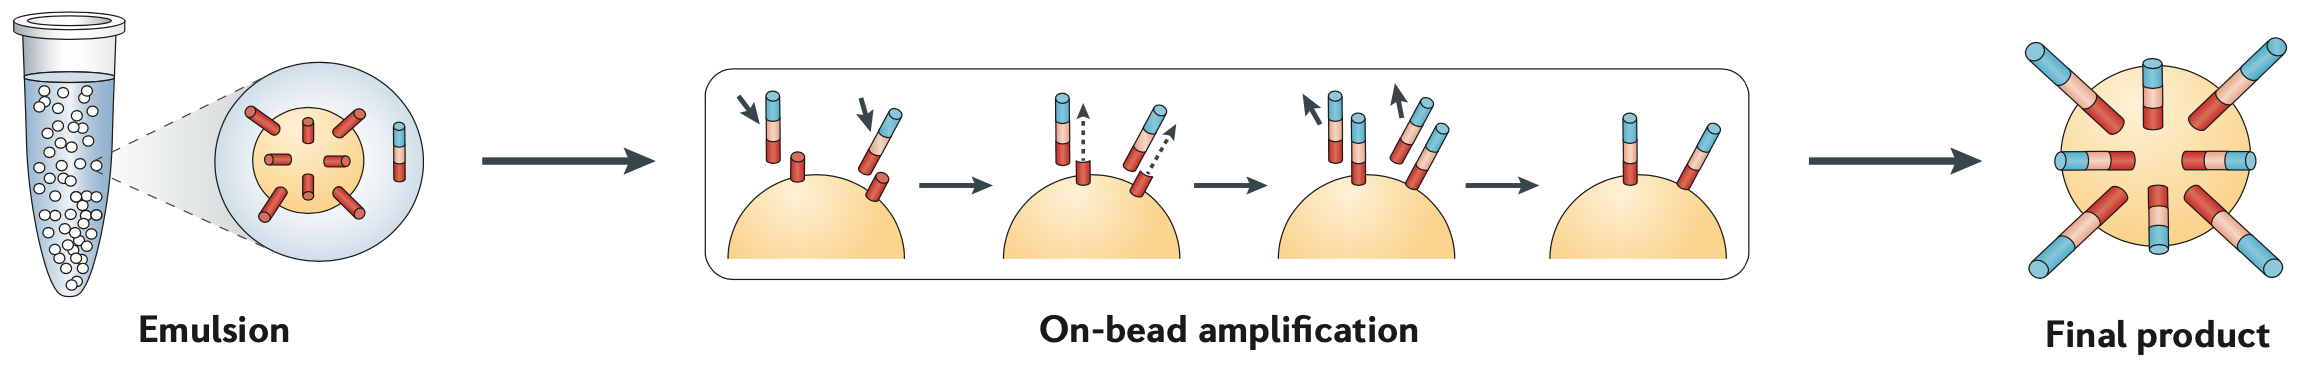
\includegraphics[width=\textwidth]{Images/chapter_3/ePCR.png}
    \caption{Ion Torrent NGS template preparation \cite{NGS}.}
    \label{fig:ePCR}
\end{figure}

For both template preparation and chip loading, the Ion Chef\texttrademark{} System (Thermo Fisher, Palo Alto, CA, USA) was used. It automates these processes, loading up to 8 samples on a single Ion 550\texttrademark{} Chip (Thermo Fisher, Palo Alto, CA, USA), which is subsequently used for sequencing.

\subsection{Sequencing}

The previously loaded chips were sequenced on an Ion GeneStudio\texttrademark{} S5 Sequencer (Thermo Fisher, Palo Alto, CA, USA). It is a semiconductor-based NGS platform that decodes the template DNA sequence by detecting \ce{H^{+}} ions that are released upon the incorporation of nucleotides to the DNA fragment attached to its corresponding bead. 

\begin{figure}[ht]
    \centering
    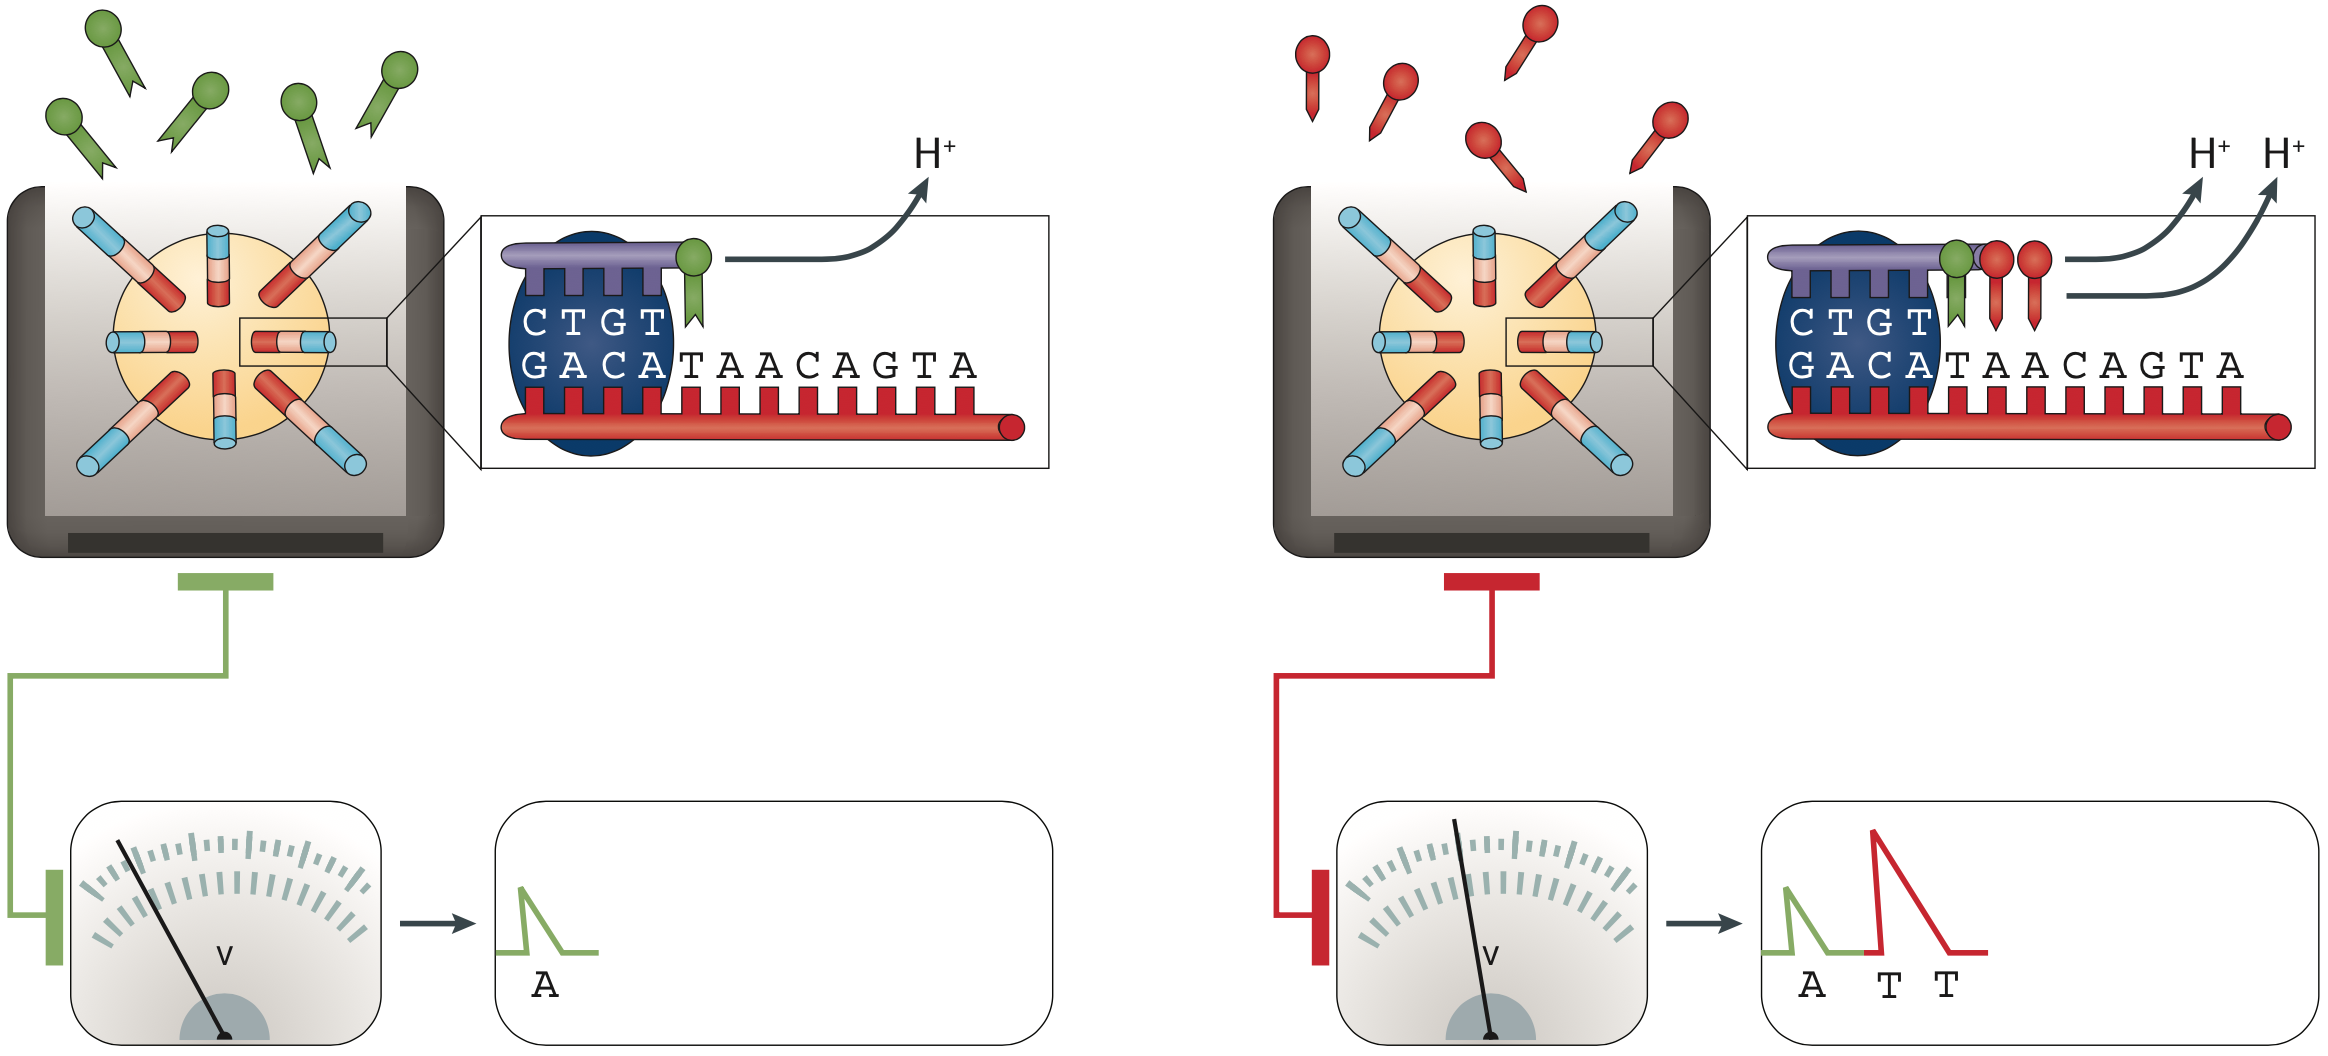
\includegraphics[width=\textwidth]{Images/chapter_3/NGS_sequencing.png}
    \caption{Ion Torrent NGS sequencing: measurement of nucleotide addition \cite{NGS}.}
    \label{fig:NGS_sequencing}
\end{figure}

This process occurs simultaneously in millions of wells, which contain template-attached beads incubated with DNA polymerase and a particular type of dNTP. Therefore, if that specific dNTP matches the growing template strand, the DNA polymerase adds it, resulting in a discharge of a \ce{H^{+}} ion that will change the pH of the solution in the well. This shift is recorded and converted to voltage, indicating that the nucleotide was incorporated and the base was called (\autoref{fig:NGS_sequencing}).

\subsection{Sequenced Data Analysis}

Data analysis was completed in two consecutive steps. First, a primary analysis was performed to study the overall quality of the sequenced data. Subsequently, the identified genetic variants were analyzed and verified using several software tools.

\subsubsection{Primary Analysis}

The sequencing runs were scheduled with the Torrent Suite\texttrademark{} v5.10 software, generating at the end of the process a file with the main quality specifications (\autoref{fig:20200108_1}), which include:
\begin{itemize}
    \item \textbf{ISP loading density}. Percentage of chip wells that contain an Ion Sphere\texttrademark{} Particle.
    \item \textbf{Total reads}. The total number of readings associated with a specific barcode.
    \item \textbf{Read length ($\boldsymbol{bp}$)}. Length of the called reads.
\end{itemize}

\begin{figure}[ht]
    \centering
    \begin{subfigure}{0.85\textwidth}
        \centering
        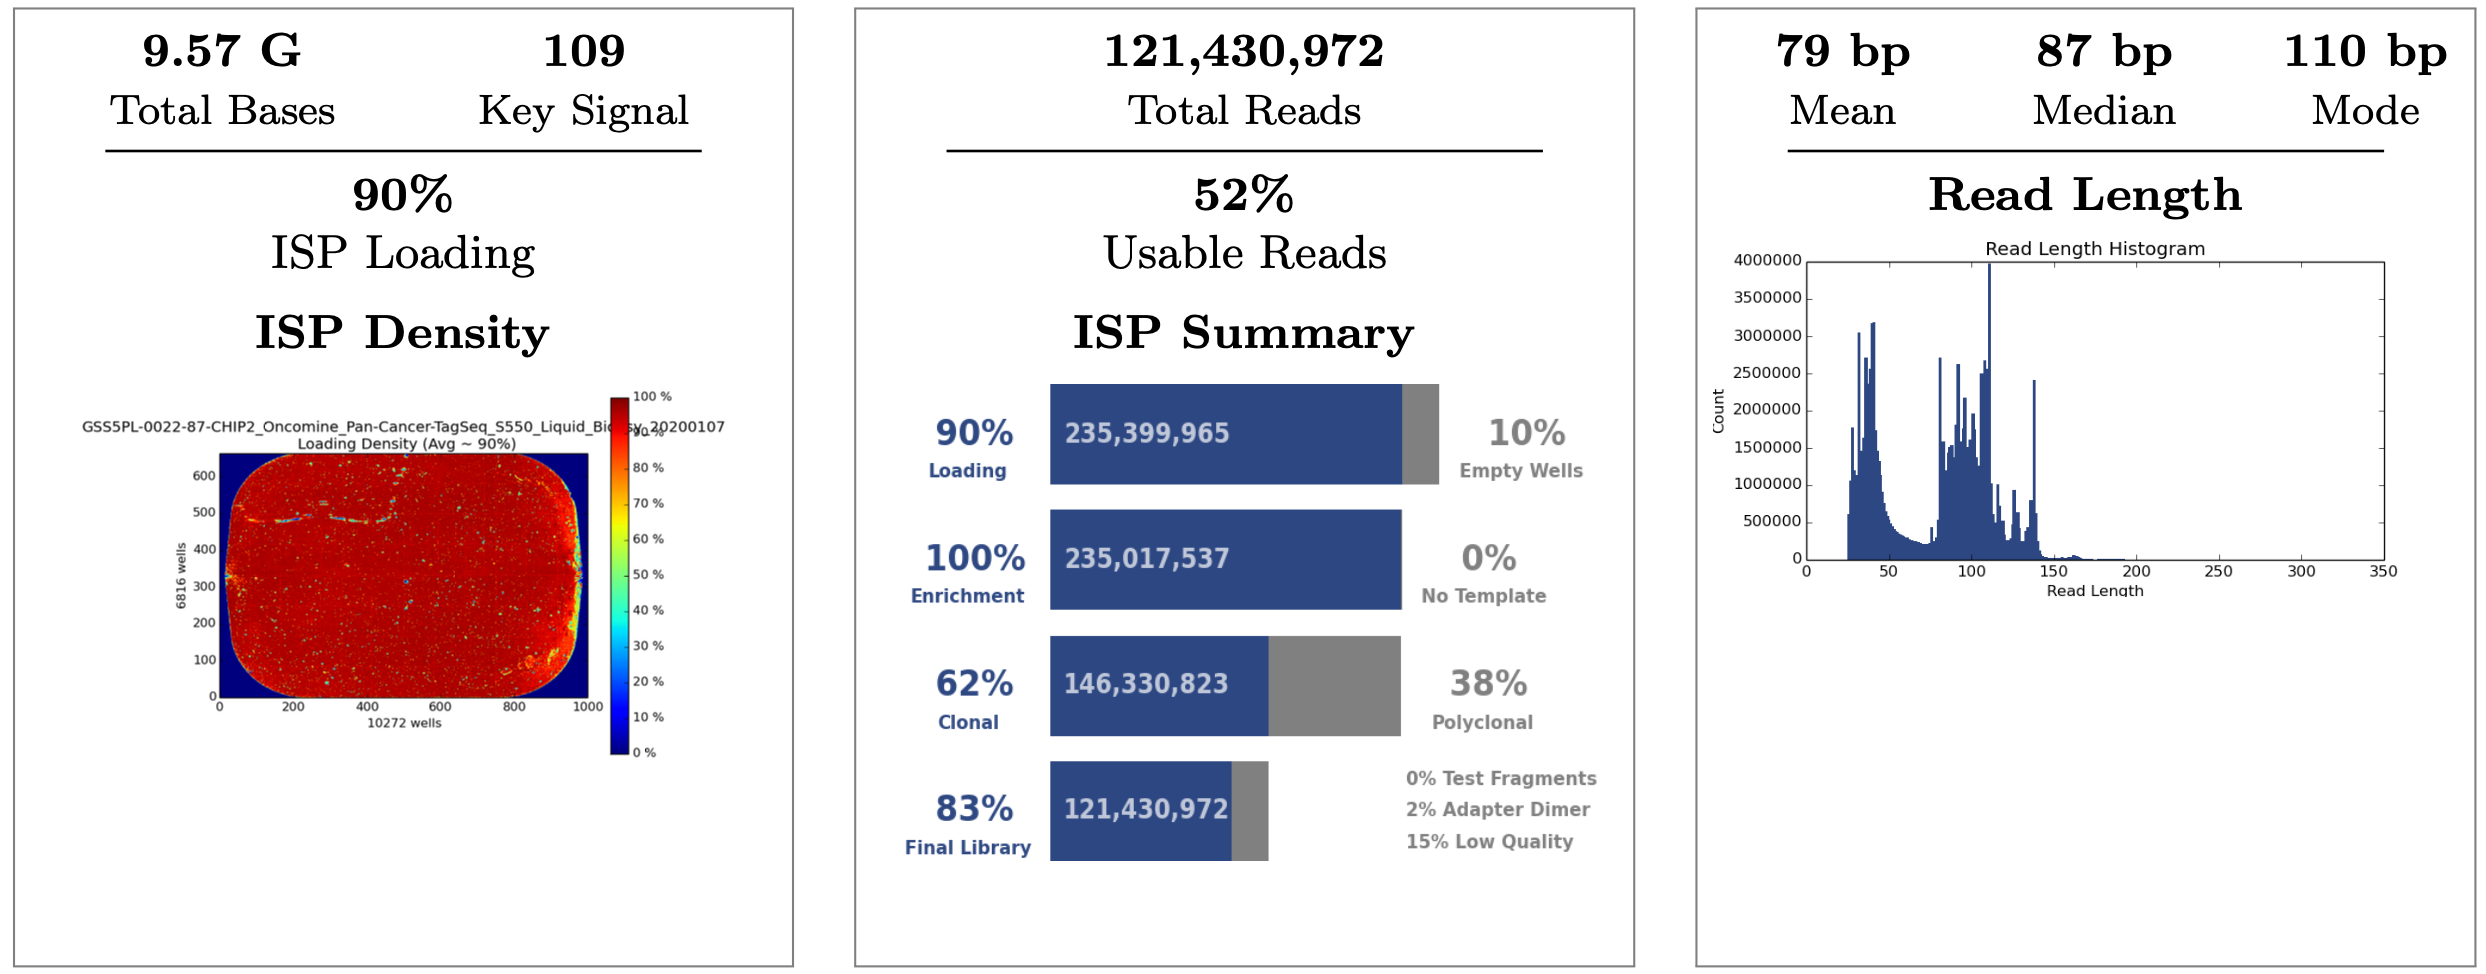
\includegraphics[width=\textwidth]{Images/chapter_3/20200108/20200108_1.png}
        \caption{Quality overview of a specific NGS run. The sequencing quality is directly proportional to the value of the ISP loading parameter. \\}
        \label{fig:20200108_1}
    \end{subfigure}
    \hfill
    \begin{subfigure}{0.85\textwidth}
        \centering
        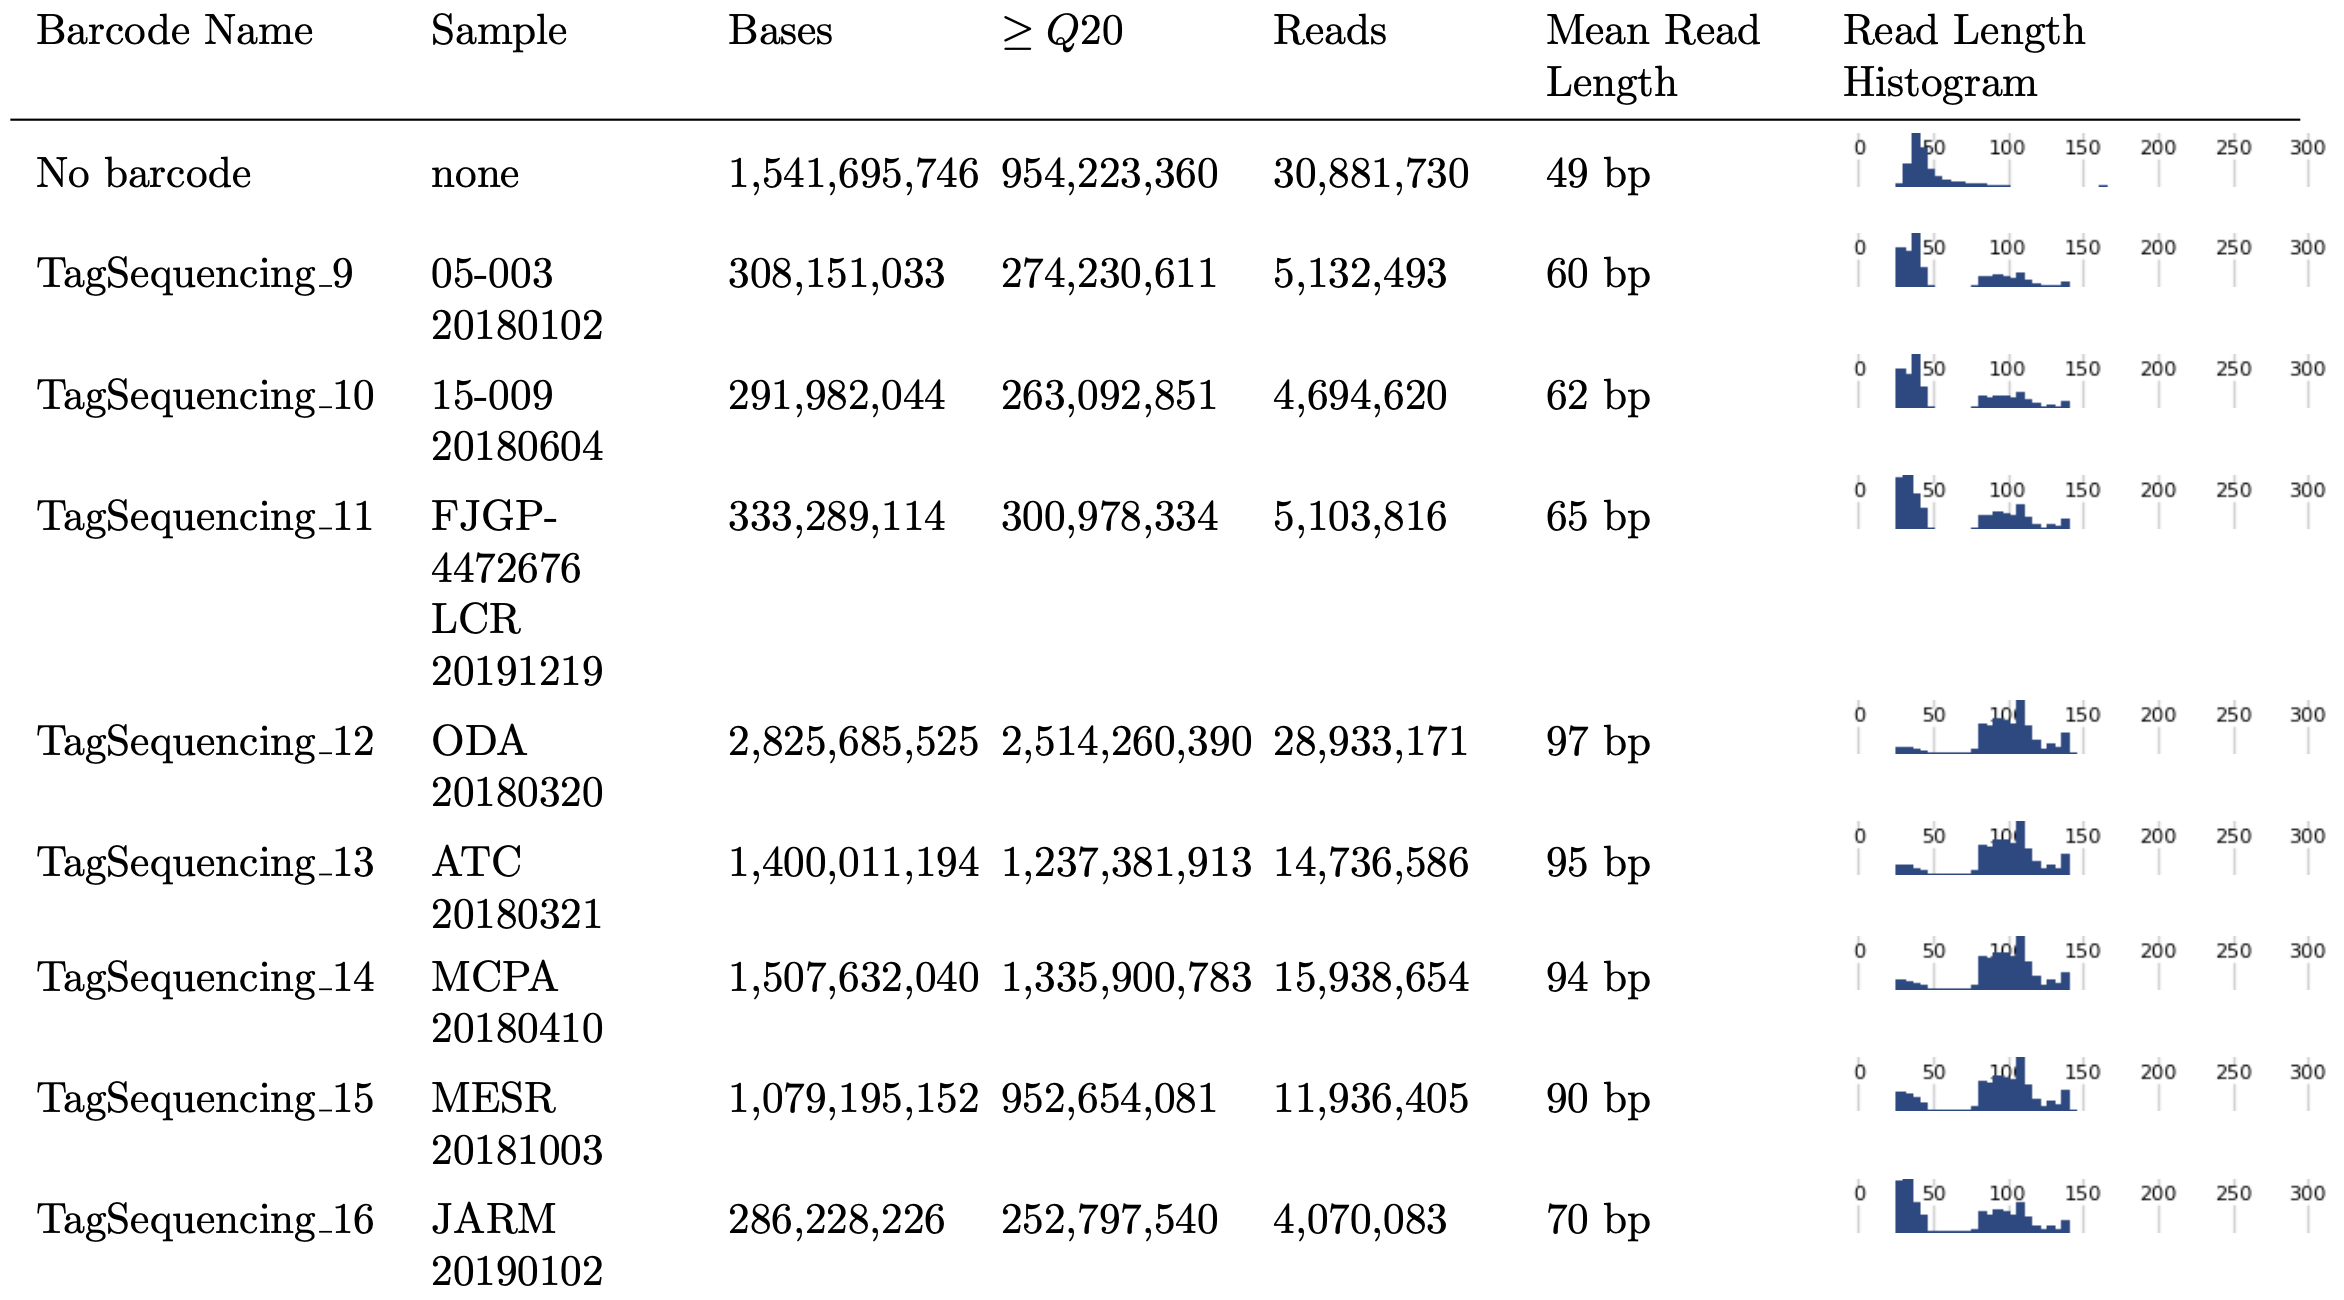
\includegraphics[width=\textwidth]{Images/chapter_3/20200108/20200108_2.png}
        \caption{Quality parameters of 8 sequenced samples. A Gaussian  base pair distribution in each of the histograms is indicative of well-prepared libraries.}
        \label{fig:20200108_2}
    \end{subfigure}
    \hfill
    \caption{Ion Torrent NGS run summary (NGS run ID: 20200108).}
    \label{fig:NGS_summary}
\end{figure}

Additionally, for each of the samples analyzed in the run (8 samples), the server generates an additional report with the following parameters (\autoref{fig:20200108_2}):
\begin{itemize}
    \item \textbf{Bases}. The number of base additions for each barcode.
    \item \textbf{$\boldsymbol{\ge}$ Q20}. The number of reads that have a predicted quality score of Q20 or better.
    \item \textbf{Reads}. The total number of filtered and trimmed library reads.
    \item \textbf{Mean read length ($\boldsymbol{bp}$)}. Average read length.
\end{itemize}

This raw data was processed automatically on the Torrent Server\texttrademark{} v5.10 and then aligned to the reference hg19 genome. In this context, to study the sequence coverage for target genomic regions, the  Coverage Analysis Plugin v5.10.0.1 software was used, obtaining the following parameters (\autoref{fig:20200108_4}):
\begin{itemize}
    \item \textbf{Mapped reads}. The total number of reads that were mapped to the reference.
    \item \textbf{On target (\%)}. Percent of reads that were mapped to any targeted region.
    \item \textbf{Mean depth}. The average number of reads that align to known reference bases.
    \item \textbf{Uniformity (\%)}. Percentage of bases, in all targeted regions, that is covered by at least 20\% of the average base coverage depth reads.
\end{itemize}

\begin{figure}[ht]
    \centering
    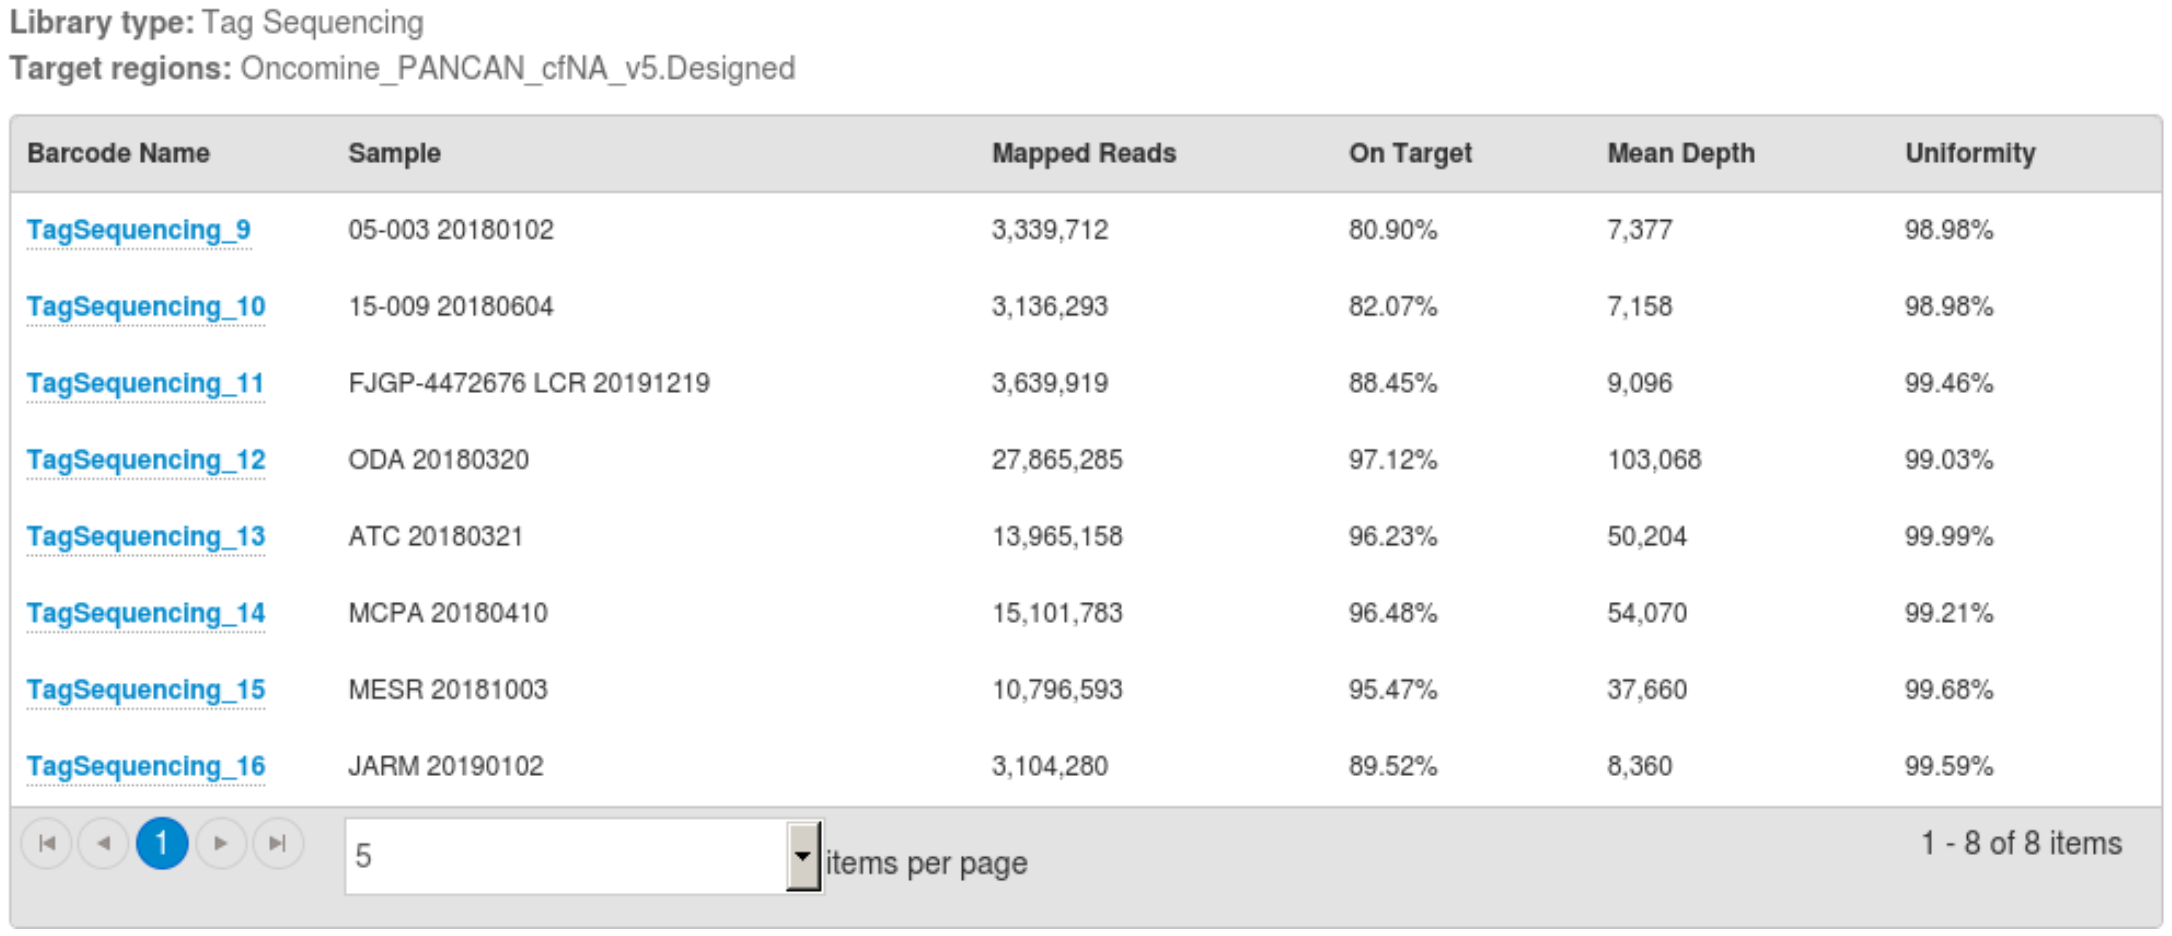
\includegraphics[width=\textwidth]{Images/chapter_3/20200108/20200108_4.png}
    \caption{Coverage Analysis Plugin output parameters of 8 sequenced samples (NGS run ID: 20200108). Successful sequencing shows a percentage of readings mapped to target regions and uniformity values close to 100\%.}
    \label{fig:20200108_4}
\end{figure}

\subsubsection{Secondary Analysis}

After ensuring that the sequencing had been performed as expected, the resulting data of the quality control passing samples were uploaded in BAM format to the Ion Reporter\texttrademark{} v5.10. Variant calling, annotation, and filtering was performed on this platform using the Oncomine\texttrademark{} TagSeq Pan-Cancer Liquid Biopsy v2.1 workflow, including this pipeline analysis the mapping of the sequenced reads to defined target regions (Oncomine\texttrademark{} Pan-Cancer DNA Regions v$1.0$) and the variant calling using the Oncomine\texttrademark{} Variant Annotator v2.3 plugin. In this context, with Ion Reporter\texttrademark{} it is possible to identify deviations from a reference genome based on their biological and clinical relevance, obtaining information about the gene, the location, the allele frequency, and the specific type of each variant.

Finally, all candidate mutations were manually reviewed using the Integrative Genomics Viewer (IGV) v2.3.40 to be subsequently confirmed by dPCR.

\subsection{Confirmation of the Sequenced Results}

Digital PCR is a tool that is used to improve the efficiency of the NGS workflow and for the verification of sequencing data. In this study, the previously identified mutations in the cfDNA or cDNA samples were confirmed by the QuantStudio\textsuperscript\textregistered{} 3D Digital PCR System (Applied Biosystems, South San Francisco, CA, USA) according to the manufacturer's specifications. The reverse transcription of exosome RNA to synthesize cDNA was performed using the PrimeScript\texttrademark{} RT Reagent Kit (TaKaRa, Japan).

In short, dPCR is based on the fact that the random distribution of molecules in many partitions follows a Poisson distribution. Each partition, which contains a specific labeled DNA sequence, acts as an individual and isolated PCR reaction. After amplification, the amplified target sequences are detected by fluorescence, which is sufficient to determine their concentration. In this study, this process was carried out following the next steps:
\begin{enumerate}[font=\bfseries]
    \item \textbf{Set up of the dPCR reaction}. It was performed by mixing a specific sample with the master mix and the assays, obtaining a final volume of 18 $\mu L$. Specifically, this reaction included 8.55 $\mu L$ of template cfDNA or cDNA, 9 $\mu L$ of 20X QuantStudio\texttrademark{} 3D Master Mix and 0.45 $\mu L$ of 40X TaqMan\texttrademark{} assays (predesigned TaqMan\texttrademark{} Liquid Biopsy dPCR assay and custom TaqMan\texttrademark{} assay). These assays include specific primers and labeled probes that have a fluorescent reporter dye (VIC\texttrademark{} or FAM\texttrademark{}) attached to its 5' end, and a quencher dye at its 3' end (ROX\texttrademark{}). In all assays, probes complementary to mutated and wild type DNA sequences were labeled with the FAM\texttrademark{} and VIC\texttrademark{} dye respectively.
    \item \textbf{Chip loading}. 14.5 $\mu L$ of the dPCR reaction was loaded using the QuantStudio\texttrademark{} 3D Digital PCR Chip Loader into the QuantStudio\texttrademark{} 3D Digital PCR 20K Chip v2, which has 20000 wells containing a DNA molecule that will be amplified independently in the thermocycling phase. In addition, positive and negative controls were included in each dPCR run to ensure that the primers have attached to the DNA strand and that there has been no foreign DNA contamination.
    %Load the dPCR reaction onto a QuantStudioTM 3D Digital PCR Chip, apply the lid, load the assembly with Immersion Fluid, then seal the loading port.
    \item \textbf{Thermocycling}. This process, which was divided into 3 consecutive stages, was carried out with the QuantStudio\textsuperscript\textregistered{} 3D Digital PCR System (Applied Biosystems, South San Francisco, CA, USA). The temperature, duration, and the number of cycles for each of the stages are summarized in \autoref{tab:dPCR_stages}. During the amplification stage, the Taq polymerase enzyme cleaves the aforementioned FAM\texttrademark{} and VIC\texttrademark{} bound probes, generating fluorescent signals that will be recorded and associated with specific wells on the chip in the next step.
    
    \begin{table}[ht]
        \centering
        \renewcommand{\arraystretch}{1.3}
        \begin{tabular}{ccccc}
        \rowcolor[HTML]{C0C0C0} 
        \textbf{Stage 1} & \multicolumn{2}{c}{\cellcolor[HTML]{C0C0C0}\textbf{Stage 2}} & \multicolumn{2}{c}{\cellcolor[HTML]{C0C0C0}\textbf{Stage 3}} \\
        \rowcolor[HTML]{FFFFFF} 96 \textdegree{C} & 56 \textdegree{C} & 98  \textdegree{C} & 72 \textdegree{C} & 22 \textdegree{C} \\
        \rowcolor[HTML]{EFEFEF} 10 $min$ & 2 $min$ & 30 $s$ & 10 $min$ & 30 $min$ \\
        \rowcolor[HTML]{FFFFFF} 1 cycle (hold) & \multicolumn{2}{c}{\cellcolor[HTML]{FFFFFF}40 cycles} & \multicolumn{2}{c}{\cellcolor[HTML]{FFFFFF}1 cycle (hold)}
        \end{tabular}
        \caption{Digital PCR reaction conditions used in this study for DNA denaturation, annealing, and elongation stages.}
        \label{tab:dPCR_stages}
    \end{table}
    \item \textbf{Chip reading}. After completing the thermocycling process, the chips were loaded into the QuantStudio\texttrademark{} 3D Digital PCR Instrument to read their fluorescence. This reading was performed twice to ensure that the subsequent data review is accurate and reliable.
    \item \textbf{Results interpretation}. The previously conditioned data were visualized and analyzed using the QuantStudio\texttrademark{} 3D Analysis Suite\texttrademark{} Cloud Software (\autoref{fig:FAM_VIC}). In this context, samples with a mutant allele fraction ($MAF = \frac{FAM_{copies}/\mu L}{FAM_{copies}/\mu L \ + \ VIC_{copies}/\mu L}$) equal to or higher than 0.1\% were considered positive. Additionally, the LOD was assessed for all individual assays, being lower than 0.1\% in all cases.
    
    \begin{figure}[ht]
        \centering
        \begin{subfigure}{0.30\textwidth}
            \centering
            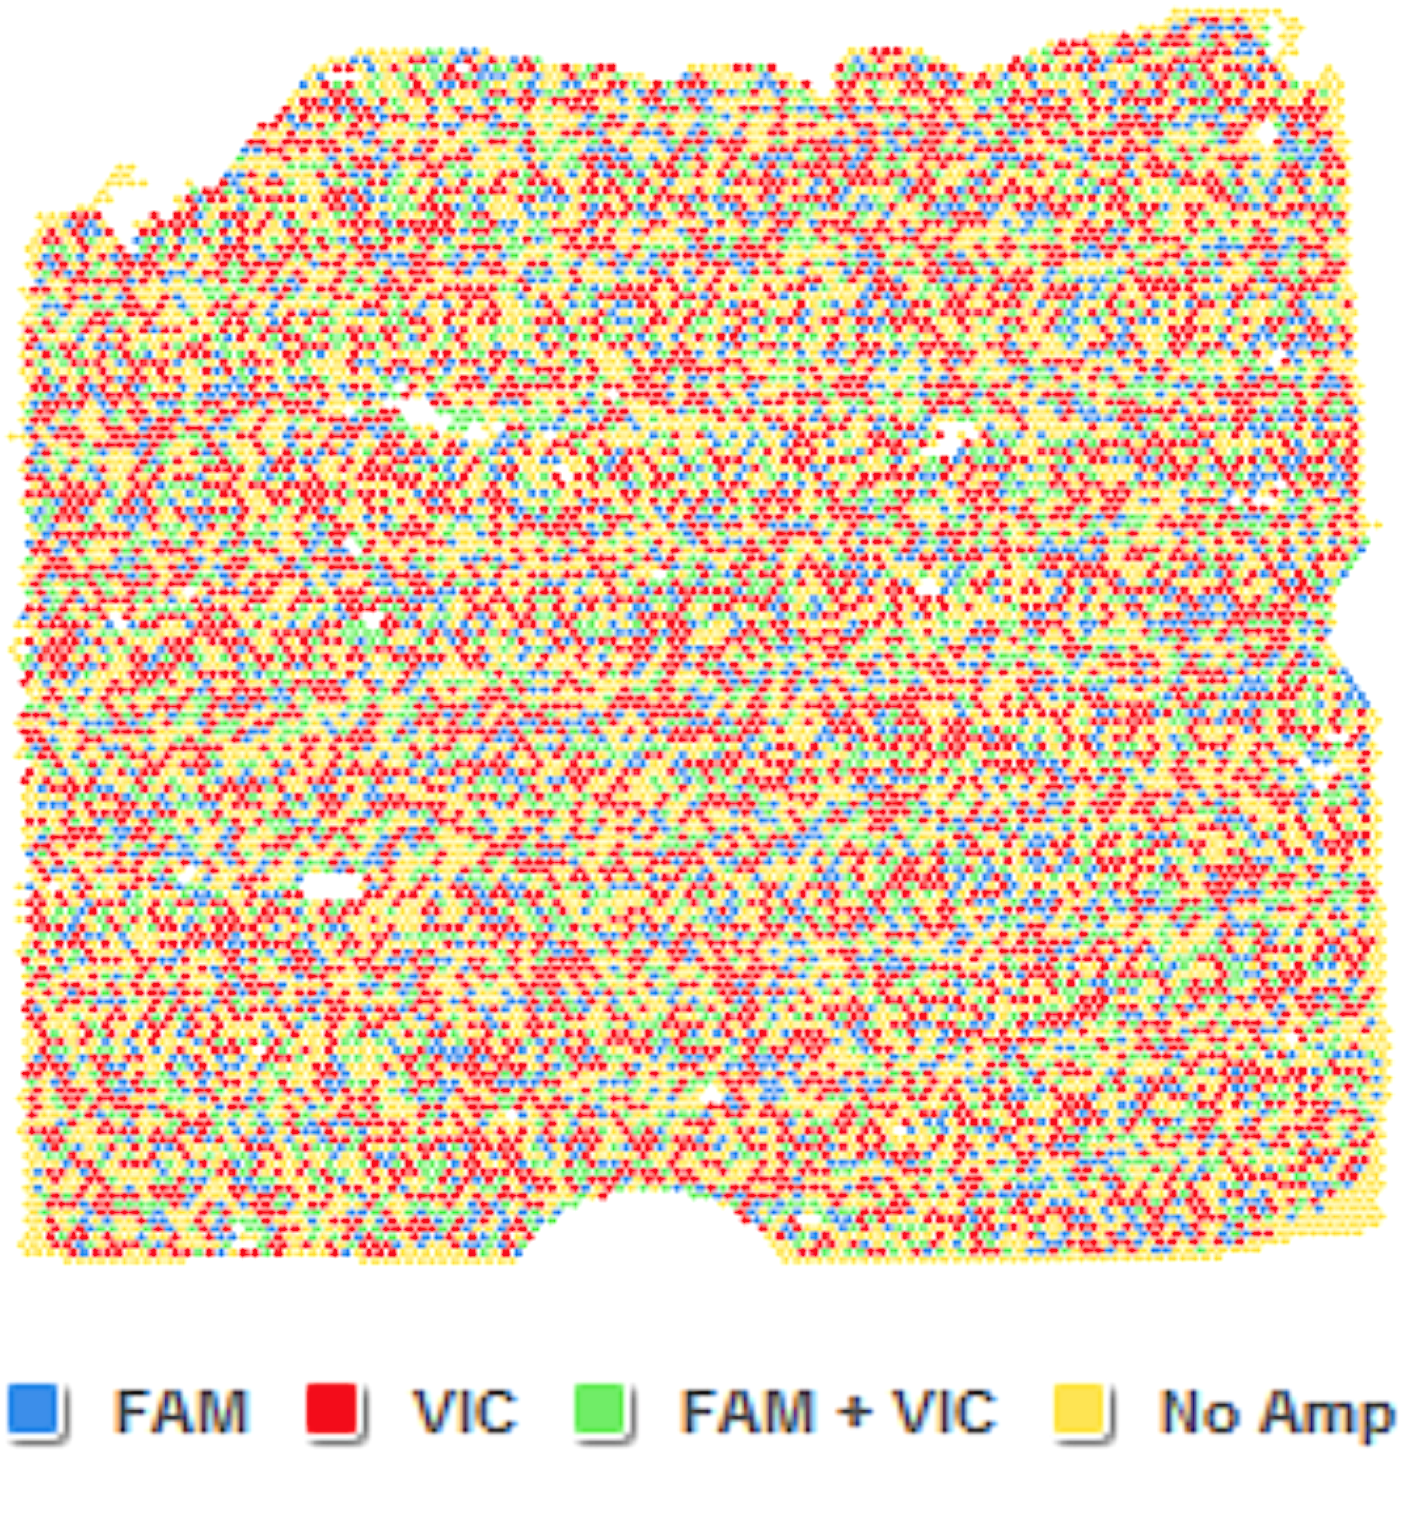
\includegraphics[width=\textwidth]{Images/chapter_3/FAM_VIC_chip.png}
            \caption{Chip view.}
            \label{fig:FAM_VIC_chip}
        \end{subfigure}
        \hfill
        \begin{subfigure}{0.69\textwidth}
            \centering
            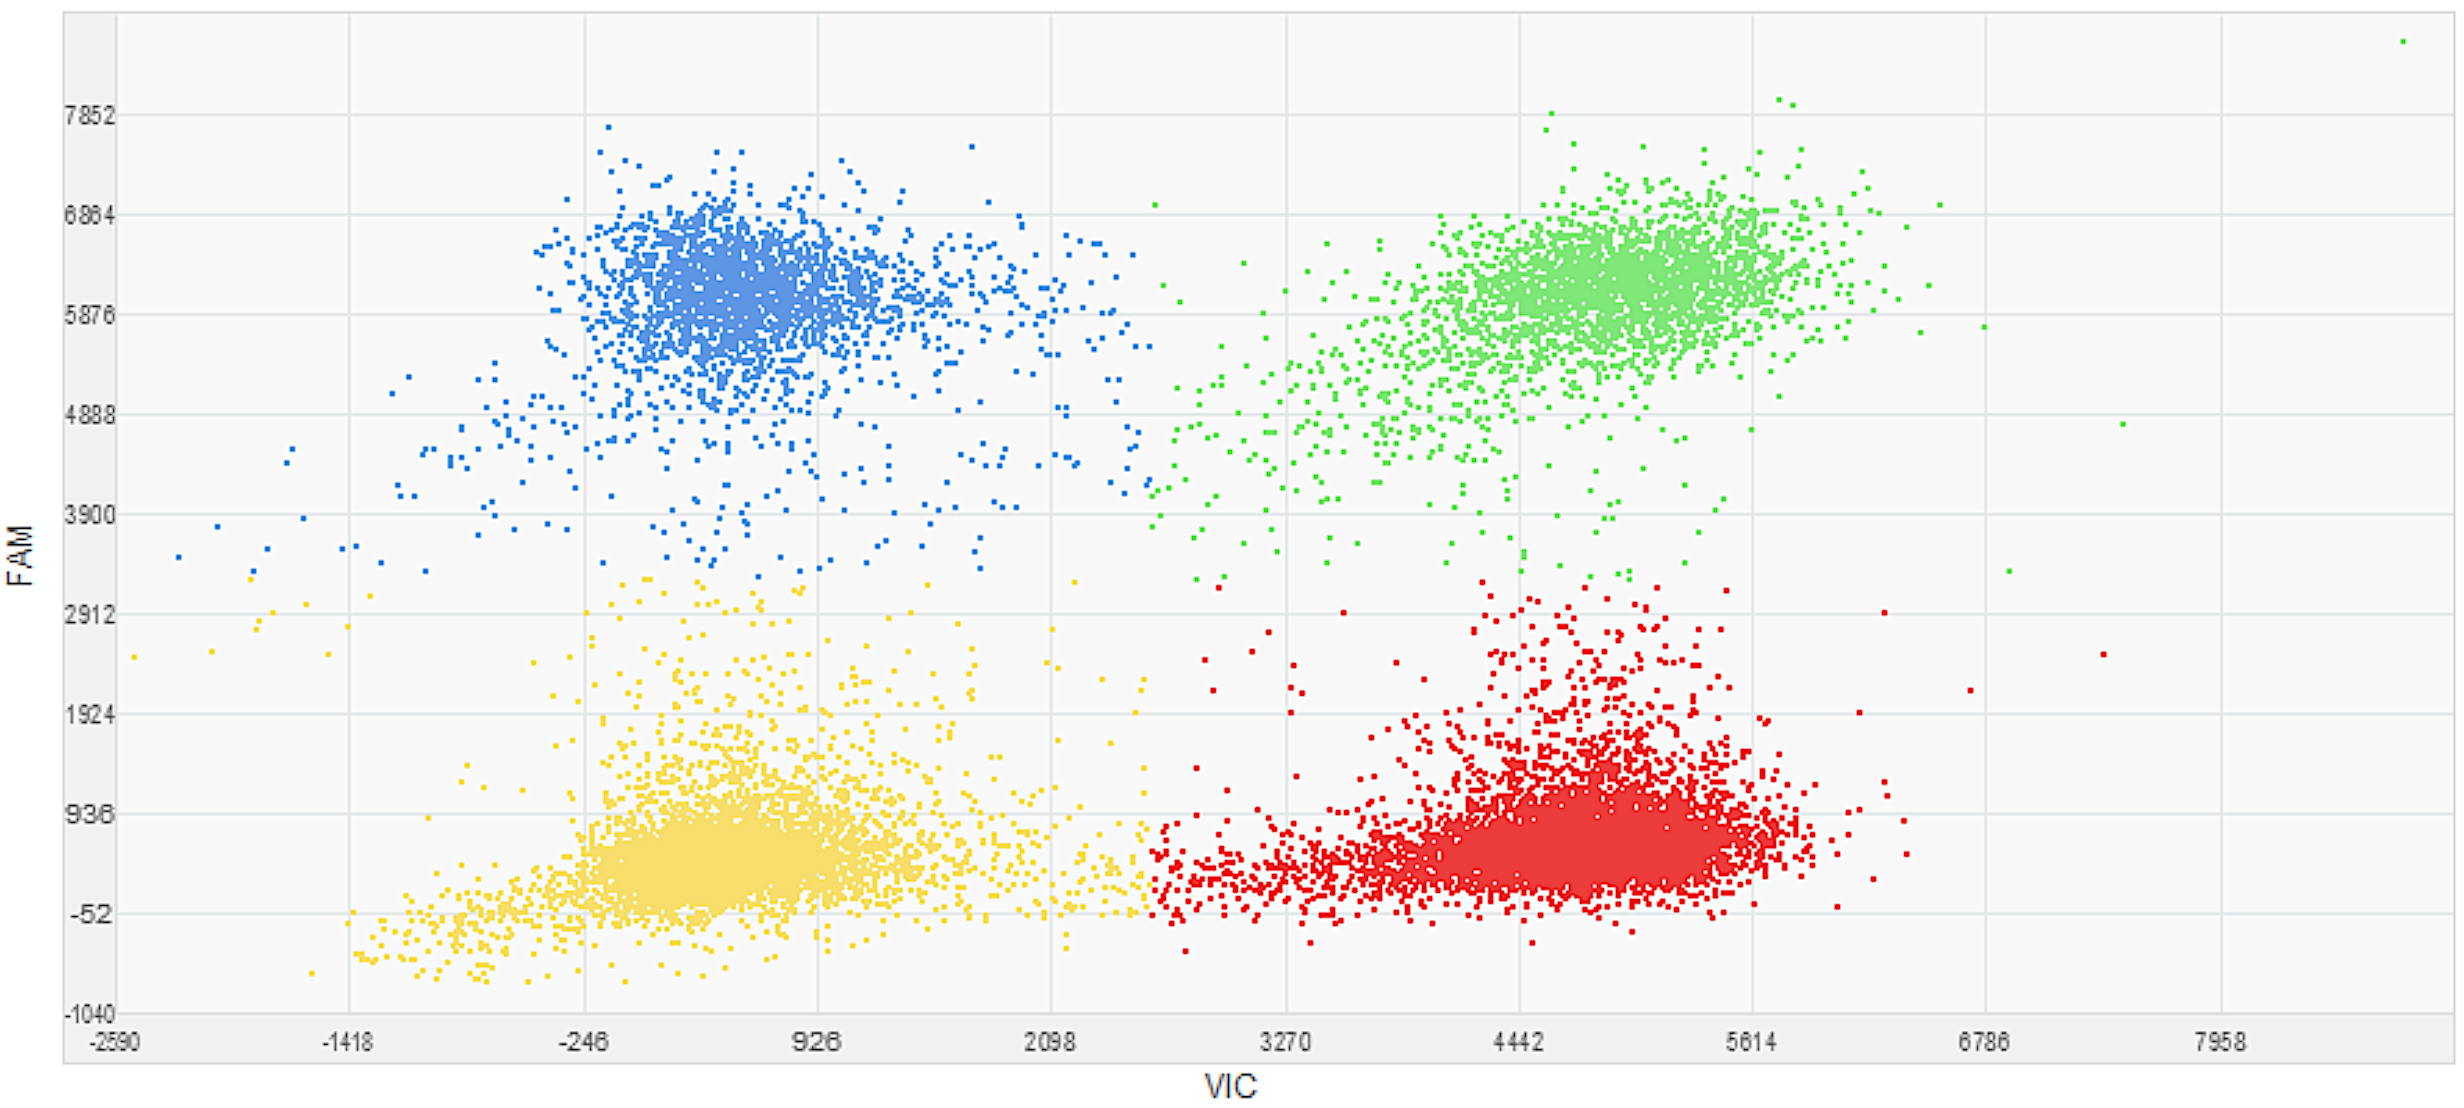
\includegraphics[width=\textwidth]{Images/chapter_3/FAM_VIC.png}
            \caption{FAM\texttrademark{} (Y-axis) vs. VIC\texttrademark{} (X-axis) view. A mutation has been detected if the blue cluster is identifiable in the dispersion chart.}
            \label{fig:FAM_VIC_dispersion}
        \end{subfigure}
        \hfill
        \caption{Quality and calls review of the dPCR. The red, blue, and green colors correspond to the VIC\texttrademark{} (fluorescence of the wild type sequences), FAM\texttrademark{} (fluorescence of the mutated sequences), and VIC\texttrademark{}+FAM\texttrademark{} groups respectively, while the yellow represents the wells without amplification.}
        \label{fig:FAM_VIC}
    \end{figure}
\end{enumerate}

\subsection{Algorithm development}



% DRIVE
% to discern whether a read of a low allele fraction represents a true mutation that exists within a subset of tumor cells or is an artifact that should be discarded.


